\section{moMoveIncrEval$<$ M $>$ Class Template Reference}
\label{classmo_move_incr_eval}\index{moMoveIncrEval@{moMoveIncrEval}}
(generally) Efficient evaluation function based a move and a solution.  


{\tt \#include $<$moMoveIncrEval.h$>$}

Inheritance diagram for moMoveIncrEval$<$ M $>$::\begin{figure}[H]
\begin{center}
\leavevmode
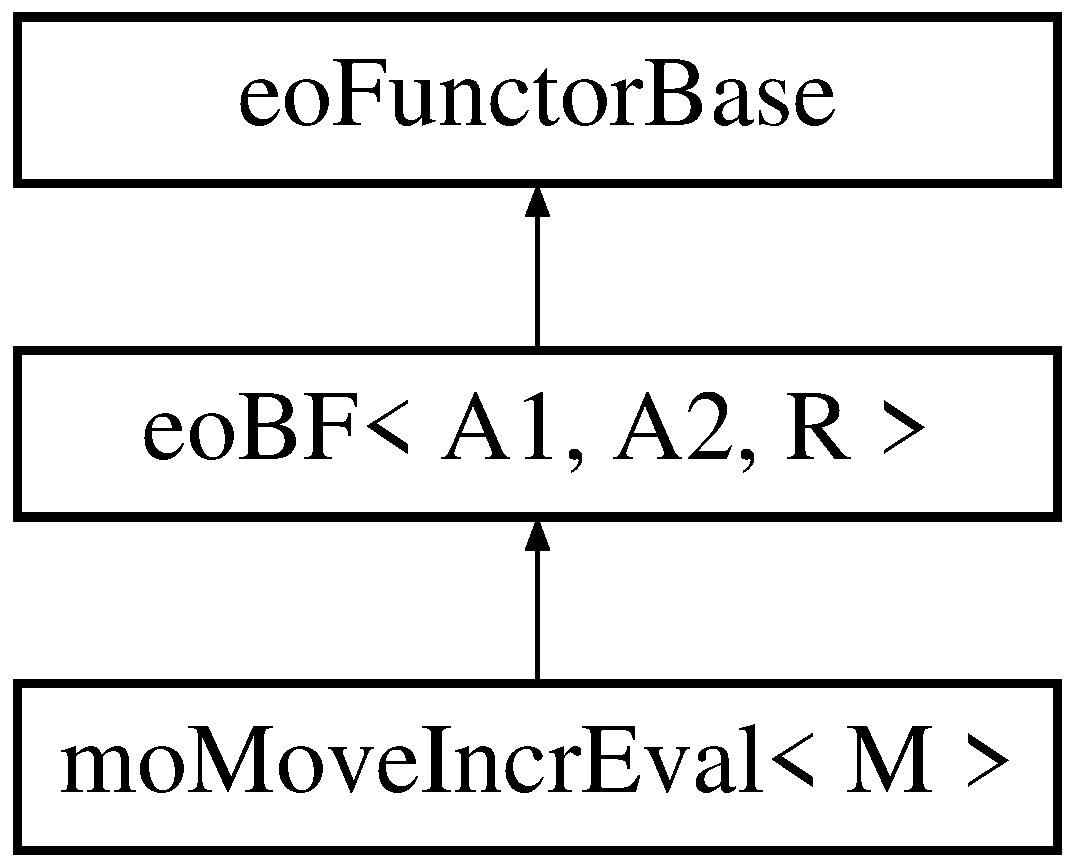
\includegraphics[height=3cm]{classmo_move_incr_eval}
\end{center}
\end{figure}


\subsection{Detailed Description}
\subsubsection*{template$<$class M$>$ class moMoveIncrEval$<$ M $>$}

(generally) Efficient evaluation function based a move and a solution. 

From a move and a solution, it computes a new fitness that could be associated to the solution if this one is updated. 

Definition at line 49 of file moMoveIncrEval.h.

The documentation for this class was generated from the following file:\begin{CompactItemize}
\item 
moMoveIncrEval.h\end{CompactItemize}
